\documentclass[11pt]{article}


%  Overall look
\usepackage[margin=0.45in]{geometry}  


% Greek
\usepackage{alphabeta}
\usepackage[utf8]{inputenc}
\usepackage[greek, english]{babel}


% Figures
\usepackage{graphicx}
\usepackage{caption}
\usepackage{subcaption}
\usepackage{float}


% Tables
\usepackage{multirow}
\usepackage{multicol}
\usepackage{booktabs}


% Math
\usepackage{amsmath}
\usepackage{amssymb}
\usepackage{mathtools}
\usepackage{wasysym}
\usepackage{steinmetz}
\usepackage{cancel}
\usepackage{bigints}
\newcommand{\eqdoub}{\overset{\mathrm{}}{=\joinrel=}}
\newcommand{\eqsix}{\overset{\mathrm{}}{=\joinrel=\joinrel=\joinrel=\joinrel=\joinrel=\joinrel}}
\newcommand{\eqeight}{\overset{\mathrm{}}{=\joinrel=\joinrel=\joinrel=\joinrel=\joinrel=\joinrel=\joinrel=}}


%code
\usepackage{listings}
\usepackage{color} %red, green, blue, yellow, cyan, magenta, black, white
\definecolor{mygreen}{RGB}{28,172,0} % color values Red, Green, Blue
\definecolor{mylilas}{RGB}{170,55,241}
\lstset{language=Python,%
	basicstyle=\small, %or \small or \footnotesize etc.
	breaklines=true,%
	frame=single,
	mathescape,
	morekeywords={matlab2tikz},
	keywordstyle=\color{blue},%
	morekeywords=[2]{1}, 
	keywordstyle=[2]{\color{black}},
	identifierstyle=\color{black},%
	stringstyle=\color{mylilas},
	commentstyle=\color{mygreen},%
	showstringspaces=false,%without this there will be a symbol in the places where there is a space
	emph=[1]{for,end,break,on,off},emphstyle=[1]\color{red}, %some words to emphasise
	numberstyle={\tiny \color{black}},% size of the numbers
	numbersep=9pt, % this defines how far the numbers are from the text
}


% For drawing
\usepackage{tikz}
\usetikzlibrary{arrows,automata,calc,shapes,backgrounds}
\usetikzlibrary{positioning} 	% For left right etc
\tikzset{
	treenode/.style = {align=center, inner sep=0pt, text centered,
		font=\sffamily},
	arn/.style = {treenode, circle, black, font=\sffamily\bfseries, draw=black,
		fill=white, text width=4.1ex},
	arnrec/.style = {treenode, rectangle, black, font=\sffamily\bfseries, draw=black,
		fill=white, text width=7.5ex,minimum width=4.0ex, minimum height=4.0ex},
	arnsmall/.style = {treenode, circle, black, font=\sffamily\bfseries, draw=black,
		fill=white, text width=1.5ex},
}
\usepackage{xcolor}
\definecolor{purple}{HTML}{9B26B6}
\usetikzlibrary{arrows.meta}
\usetikzlibrary{matrix,positioning}

% Table of contents
% Clickable
\usepackage{hyperref}
\hypersetup{
	colorlinks,
	citecolor=black,
	filecolor=black,
	linkcolor=black,
	urlcolor=black
}
% Dots
\usepackage{tocloft}
\renewcommand{\cftsecleader}{\cftdotfill{\cftdotsep}}


%First page
\newcommand{\subject}{Large and Social Networks}
\newcommand{\descript}{1o Σετ Ασκήσεων}
\newcommand{\names}{Σταυρόπουλος Αλέξανδρος Ανδρέας\\ 2019030109}
\newcommand{\lecturer}{Θρασύβουλος Σπυρόπουλος}
\newcommand{\lablecturer}{-}
\newcommand{\term}{Χειμερινό εξάμηνο 2022-2023}


% Line above page numbering
\usepackage{titleps}%
\newpagestyle{ruled}{%
	\footrule
	\setfoot{}{\thepage}{}}
\pagestyle{ruled}



% Begin Code
\begin{document}
	\begin{titlepage}
	\begin{center}
		\vspace*{1cm}
		\rule{\textwidth}{1.6pt}\vspace*{-\baselineskip}\vspace*{2pt}
		\rule{\textwidth}{0.4pt}\\[\baselineskip]
		{\LARGE{\textbf{\subject}}}\\
		\vspace{0.3cm}
		{\large\descript\\}
		\rule{\textwidth}{0.4pt}\vspace*{-\baselineskip}\vspace{3.2pt}
		\rule{\textwidth}{1.6pt}\\[\baselineskip]
				
		\vspace{1.5cm}
		\textbf{\names}
		\vspace{0.3cm}
		
		\vfill
		
		Διδάσκων:\\
		\lecturer\\
		\vspace{0.5cm}
		Υπεύθυνος εργαστηρίου:\\
		\lablecturer
		\vspace{0.8cm}
		
		
\includegraphics[width=0.3\textwidth]{Images/university}
		
		ΗΜΜΥ\\
		Πολυτεχνείο Κρήτης\\
		\term
		
	\end{center}
\end{titlepage}
	\newpage
	% Remaning and Centering ToC
	\begin{center}
		\renewcommand{\contentsname}{\centering \text{Πίνακας Περιεχομένων}}
		\tableofcontents
	\end{center}
	\newpage
	\subsubsection*{Εισαγωγή}
Στην πρώτη άσκηση ζητείται η υλοποίηση των αλγορίθμων ε-Greedy και Upper Confidence Bound, oι οποίοι επιτυγχάνουν ισορροπία μεταξύ exploration και exploitation στο γνωστό πρόβλημα κουλοχέρηδων (Bandits Problem). Εφόσον υλοποιήθηκε κάθε αλγόριθμος, δόθηκε ως όρισμα το ίδιο σύνολο από bandits ώστε να εκτελεστούν για συγκεκριμένο αριθμό γύρων (Ορίζοντας Τ) και επίσης επιλέχθηκε ένας από τους bandits με βάση τον γινόμενο μεταξύ reward και πιθανότητας επιτυχίας. Η επίδοση κάθε αλγορίθμου βασίζεται στο regret το οποίο είναι η διαφορά μεταξύ του σκορ του αρχικά επιλεγμένου bandit και του σκορ που μάζεψε ο κάθε αλγόριθμος.  

\subsubsection*{ε-Greedy}
\noindent
Στον αλγόριθμο ε-Greedy στην περίπτωση exploration επιλέγεται τυχαίο χέρι ανεξάρτητα των επιδόσεών του έως τώρα ενώ στην περίπτωση exploitation επιλέγεται το χέρι με την καλύτερη επίδοση. Η επίδοση κάθε χεριού ορίζεται μέσω του συντελεστή $\mu$ ο οποίος είναι ίσος με τον πηλίκο μεταξύ του σκορ που έχει μαζέψει το εκάστοτε χέρι προς τον αριθμό των φορών που έχει επιλεχθεί. Το σκορ προκύπτει ως το γινόμενο μεταξύ reward και διωνυμικής πιθανότητας κάθε χεριού και υπολογίζεται σε κάθε γύρο ξεχωριστά. 

\noindent\\
Η επιλογή μεταξύ exploitation και exploitation γίνεται με χρήση της μεταβλητής epsilon η οποία ορίζεται ως εξής:
\begin{equation*}
	epsilon = (t)^{-\frac{1}{3}} \cdot (k \cdot \log(t))^{\frac{1}{3}}
\end{equation*}

\noindent
Σε κάθε γύρο, με πιθανότητα epsilon γίνεται explore ενώ με πιθανότητα 1 - epsilon γίνεται exploit και λαμβάνοντας υπόψιν τον φθίνον ρυθμό της μεταβλητής epsilon, μπορεί εύκολα να αποδειχθεί πως όσο αυξάνονται οι γύροι τόσο πιο πιθανό είναι να γίνει exploitation χρησιμοποιώντας το καλύτερο χέρι ενώ ταυτόχρονα τόσο πιο απίθανο να επιλεγεί κάποιο τυχαίο (exploration). Η υλοποίηση παρουσιάζει convergence rate ίσο με:
\begin{equation}
	O\left( (t)^{\frac{2}{3}} \cdot (K \cdot \log(t))^{\frac{1}{3}} \right)
\end{equation}



\subsubsection*{Upper Confidence Bound}
\noindent
Στον αλγόριθμο Upper Confidence Bound (UCB) η επιλογή χεριού γίνεται με βάση τον συντελεστή ubc:
\begin{equation*}
	ucb = \mu + \sqrt{\frac{\log T}{Q} }
\end{equation*}

όπου $\mu$ ο συντελεστής επίδοσης κάθε χεριού, Τ ο ορίζοντας και Q οι φορές που έχει επιλεχθεί το αντίστοιχο χέρι.

\noindent\\
Σε κάθε γύρο επιλέγεται το χέρι το οποίο παρουσιάζει μεγαλύτερο συντελεστή ucb κάτι το οποίο προκύπτει είτε λόγο καλής επίδοσης (συντελεστής $\mu$) είτε επειδή έχουν περάσει πολλοί γύροι που δεν έχει επιλεχθεί το εκάστοτε χέρι. Αυτό έχει ως αποτέλεσμα, το exploration πρακτικά να μην σταματάει ποτέ καθώς ακόμα και για μεγάλο αριθμό γύρου, ανά διαστήματα επιλέγεται διαφορετικό χέρι και αξιολογείται εκ νέου το performance του κάτι το οποίο στον ε-Greedy είναι σχεδόν απίθανο να συμβεί.  Η υλοποίηση παρουσιάζει convergence rate ίσο με:
\begin{equation}
	O\left( \sqrt{K \cdot T \cdot \log T}\right)
\end{equation}


\subsubsection*{Σύγκριση επιδόσεων}
\begin{minipage}{.7\textwidth}
	Εξετάζοντας τα convergence rate κάθε αλγορίθμου αναμένεται η επίδοση του UCB να είναι καλύτερη σε σχέση με του ε-Greedy. Για την επαλήθευση αυτής της εκτίμησης, έγινε σύγκριση των επιδόσεων μεταξύ των δύο αλγορίθμων για το ίδιο σετ bandits σε κάθε τεστ. Αρχικά, για 10 bandits και ορίζοντα μεγέθους 1000, τα αποτελέσματα που εξάχθηκαν δεν συναδουν πάντα με την εκτίμηση. Συχνότερη περίπτωση αποτελεί, όπως ήταν αναμενόμενο, ο UCB να παρουσιαζει καλύτερο performance δηλαδή μικρότερο regret (fig:\ref{fig:UCB_1000}), ωστόσο, υπήρξαν σπάνιες περιπτώσεις όπου ο ε-Greedy παρουσίασε καλύτερη επίδοση (fig:\ref{fig:epsilon_1000}) κάτι το οποίο είναι πιθανό να συμβεί καθώς το σκορ κάθε αλγορίθμου υπολογίζεται ξεχωριστά οπότε για τυχαίους λόγους ο ένας αλγόριθμος να είναι πολύ πιο "τυχερός" από τον άλλο. \end{minipage}
\begin{minipage}{.3\textwidth}
asdfasfasdfads
\end{minipage}

\begin{figure}[h]
	\centering
	\begin{minipage}{.33\textwidth}
	  \centering
	  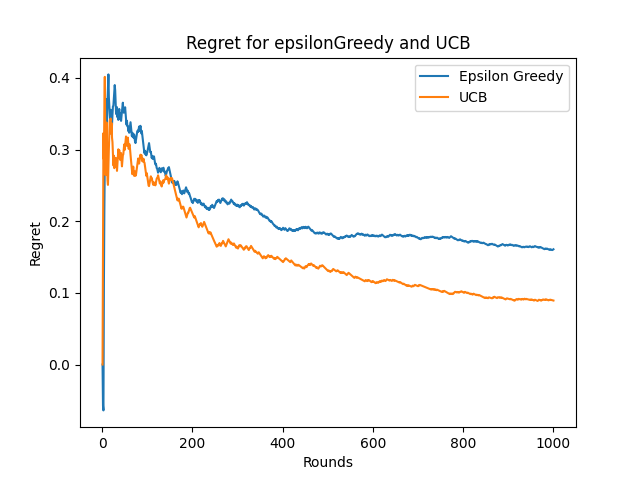
\includegraphics[width=\linewidth]{Images/regret_1000_UCB.png}
	  \captionof{figure}{Lower regret for UCB}
	  \label{fig:UCB_1000}
	\end{minipage}%
	\begin{minipage}{.33\textwidth}
	  \centering
	  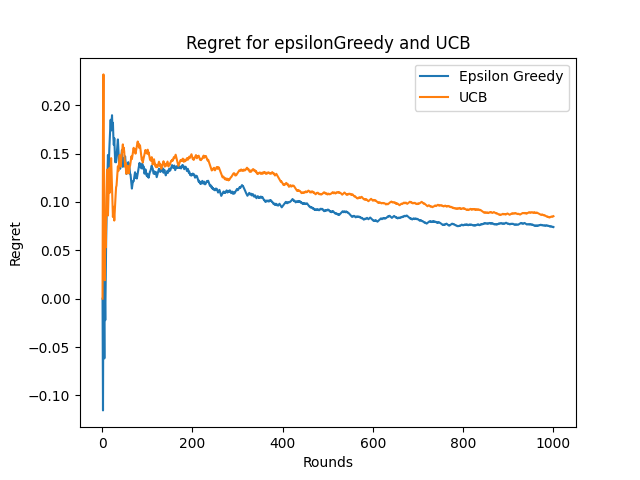
\includegraphics[width=\linewidth]{Images/regret_1000_epsilon.png}
	  \captionof{figure}{Lower regret for ε-Greedy}
	  \label{fig:epsilon_1000}
	\end{minipage}
	\begin{minipage}{.33\textwidth}
		\centering
		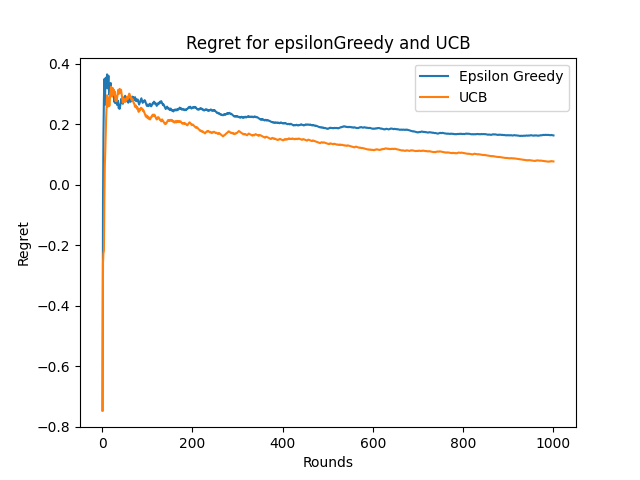
\includegraphics[width=\linewidth]{Images/regret_1000_100.png}
		\captionof{figure}{Mean value of regret}
		\label{fig:epsilon_1000_100}
	  \end{minipage}
	\end{figure}

\noindent
Για την καλύτερη επιβεβαίωση των αποτελεσμάτων, αρχικά αυξήθηκε η τιμή ορίζοντα (Τ = 10000) ενώ ο αριθμός των bandit παρέμεινε σταθερός. Στην περίπτωση αυτή ο UCB πάντα παρουσιάζει καλύτερη επίδοση, δηλαδή μικρότερο regret, σε σχέση με τον ε-Greedy κάτι το οποίο επιβεβαιώνει την αρχική εκτίμηση 

\begin{figure}[h]
	\centering
	\begin{minipage}{.33\textwidth}
	  \centering
	  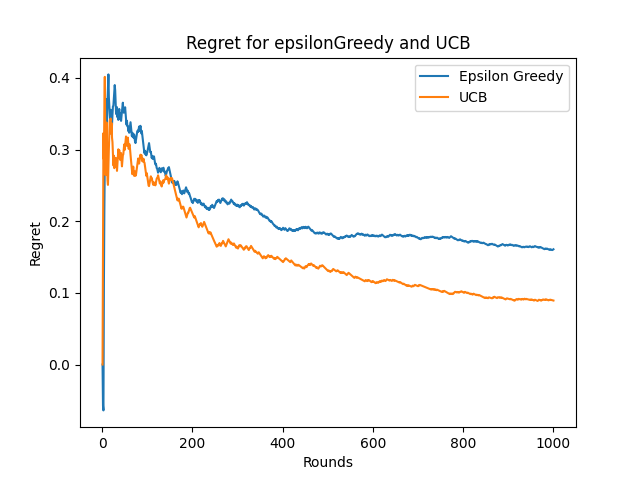
\includegraphics[width=\linewidth]{Images/regret_1000_UCB.png}
	  \captionof{figure}{Lower regret for UCB}
	  \label{fig:UCB_10000}
	\end{minipage}%
	\begin{minipage}{.33\textwidth}
	  \centering
	  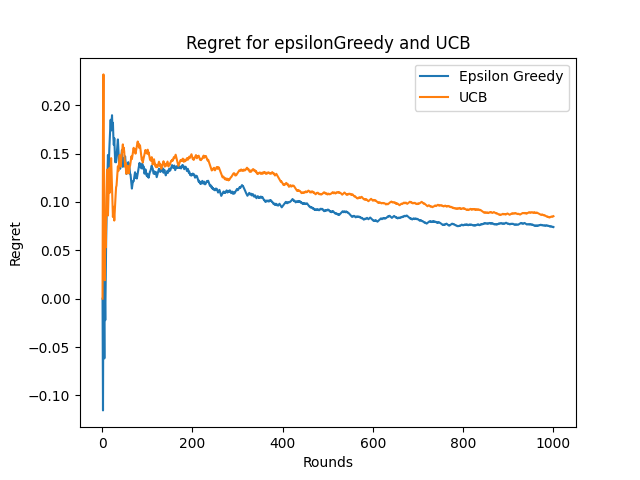
\includegraphics[width=\linewidth]{Images/regret_1000_epsilon.png}
	  \captionof{figure}{Lower regret for ε-Greedy}
	  \label{fig:epsilon_10000}
	\end{minipage}
	\begin{minipage}{.33\textwidth}
		\centering
		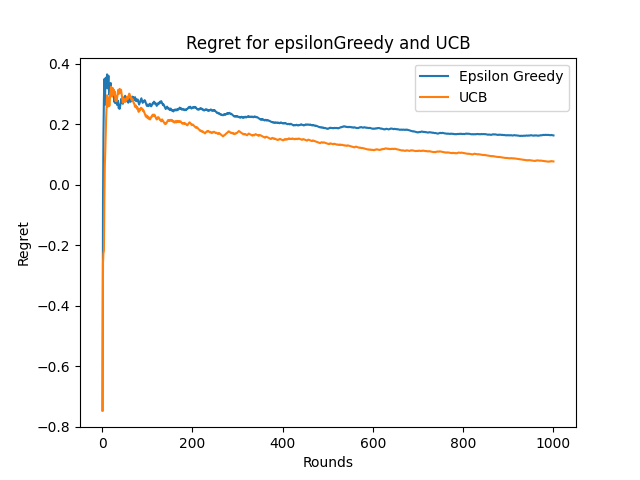
\includegraphics[width=\linewidth]{Images/regret_1000_100.png}
		\captionof{figure}{Mean value of regret}
		\label{fig:epsilon_10000_100}
	  \end{minipage}
	\end{figure}


\clearpage



\begin{itemize}
	\item πες οτι ο άλλος είναι πιο απλός και δεν βγάζει τόσο κακά αποτελέσματα
\end{itemize}
	\section*{Άσκηση 2}
\label{ex2}
\addcontentsline{toc}{section}{\nameref{ex2}}

\subsection*{Ερώτημα 1}
\label{ex2q1}
\addcontentsline{toc}{subsection}{\nameref{ex2q1}}

Σύμφωνα με τα δεδομένα της εκφώνησης η Discrete Time Markov Chain σχεδιάζεται ως εξής:\\\\

\begin{figure}[!h]
	\begin{center}
		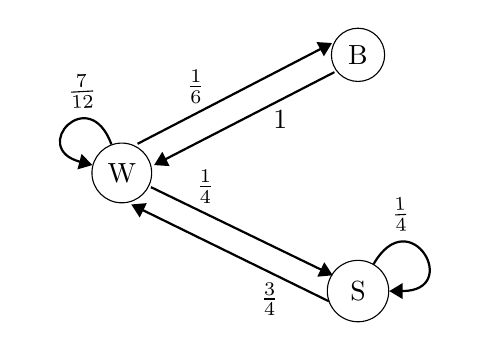
\begin{tikzpicture}
			\node [circle,draw, minimum size=0.5cm] at (2,  0) (W) {W};
			\node [circle,draw, minimum size=0.78cm] at (5, -1.5) (S) {S};
			\node [circle,draw, minimum size=0.5cm] at (5,  1.5) (B) {B};

			\draw [-Triangle, thick] ($(W) + (0.2, 0.37)$) -- ($(B) + (-0.33, 0.15)$) node [pos=0.3, above] {$\frac{1}{6}$};
			\draw [-Triangle, thick] ($(B) + (-0.3, -0.22)$) -- ($(W) + (0.41, 0.1)$) node [pos=0.3, below] {1};
			
			\draw [-Triangle, thick] ($(W) + (0.37, -0.18)$) -- ($(S) + (-0.32, 0.2)$) node [pos=0.3, above] {$\frac{1}{4}$};
			\draw [-Triangle, thick] ($(S) + (-0.37, -0.13)$) -- ($(W) + (0.12, -0.4)$) node [pos=0.3, below] {$\frac{3}{4}$};

			\path (S) edge [loop right, thick, -Triangle, in=0, out=60, looseness=6] node [above, sloped, pos=0.25] (TextNode1) {$\frac{1}{4}$} (S);
			\path (W) edge [loop right, thick, -Triangle, in=165, out=110, looseness=6] node [above, sloped, pos=0.32] (TextNode1) {$\frac{7}{12}$} (W);
		\end{tikzpicture}
	\end{center}
	\caption{Discrete Markov Chain}
	\label{DTMC}
\end{figure}

\subsection*{Ερώτημα 2}
\label{ex2q2}
\addcontentsline{toc}{subsection}{\nameref{ex2q2}}

Για να είναι εργοτική η DTMC του figure 3 είναι απαραίτητο να ισχύουν οι εξής προϋποθέσεις:
\begin{enumerate}
	\item Recurrent (Ελληνικά)
	\item Απεριοδική
	\item All nodes communicating to each other
\end{enumerate}

\noindent\\
\textbf{Recurrent}\\
H DTMC είναι Recurrent εφόσον δεν υπάρχει κάποιο state το οποίο είναι transient, δηλαδή δεν υπάρχει κάποιο state από το οποίο αν γίνει μετάβαση από αυτό, δεν είναι εφικτή η επιστροφή σε αυτό.\\

\noindent\\
\textbf{Απεριοδικότητα}\\
Η DTMC είναι Απεριοδική εφόσον δεν υπάρχει κάποιο state το οποίο είναι περιοδικό, δηλαδή δεν υπάρχει κάποιο state από το οποίο όλα τα πιθανά μονοπάτια που ξεκινούν και καταλήγουν σε αυτό να είναι πολλαπλάσια του ίδιου αριθμού Κ (Κ$>$1). Αυτό συμβαίνει καθώς υπάρχουν self loops σε 2 από τα 3 states με αποτέλεσμα η μετάβαση να μπορεί να μεγαλώσει αρκετά αξιοποιώντας τα.\\

\noindent
π.χ. για το state Β, η μετάβαση $B \xrightarrow[]{} W \xrightarrow[]{} B$ έχει ελάχιστο μήκος διαδρομής, ίσο με 2, όμως αντίστοιχα μπορεί\\ \vspace{1cm} \qquad να εκτελεστεί και η διαδρομή $B \xrightarrow[]{} W \xrightarrow[]{} W \xrightarrow[]{} B$ η οποία έχει μήκος ίσο με 3.

\noindent
\textbf{All nodes connect with each other}\\
Από το figure (\ref{DTMC}) είναι εμφανές πως όλοι οι κόμβοι επικοινωνούν μεταξύ τους, δηλαδή από κάθε ένα κόμβο, μπορεί να γίνει μετάβαση σε έναν άλλο.


\noindent\\\\\\
Άρα, πληρούνται όλες οι προϋποθέσεις και ως αποτέλεσμα η DTMC είναι εργοτική

\clearpage
\subsection*{Ερώτημα 3}
\label{ex2q3}
\addcontentsline{toc}{subsection}{\nameref{ex2q3}}

Για να είναι χρονικά-αναστρέψιμη η DTMC πρέπει να ισχύει το local balance. Εφαρμόζοντας local balance σε κάθε ζευγάρι κόμβων προκύπτουν οι εξής σχέσεις:
\begin{align}
	P_W \cdot \frac{1}{6} = P_B \cdot 1 &\xRightarrow{} P_B = P_W \cdot \frac{1}{6} \label{pbw}\\
	P_W \cdot \frac{1}{4} = P_S \cdot \frac{3}{4} &\xRightarrow{} P_S = P_W \cdot \frac{1}{3} \label{psw}
\end{align}

\noindent\\
Ακόμα, πρέπει να ισχύει η εξής σχέση:
\begin{align*}
	P_W + P_B + P_S = 1
\end{align*}

οπότε αντικαθιστώντας τις σχέσεις (\ref{pbw}), (\ref{psw}) προκύπτουν τα εξής αποτελέσματα:
\begin{align}
	P_W + P_B + P_S = 1 &\xRightarrow{} P_W + P_W \cdot \frac{1}{6} + P_W \cdot \frac{1}{3} = 1 \notag \xRightarrow{}\\
						&\xRightarrow{} P_W \left( \frac{6}{6} + \frac{1}{6} +  \frac{2}{6} \right) = 1 \notag \xRightarrow{}\\
						&\xRightarrow{} P_W \left( \frac{3}{2} \right) = 1 \notag \xRightarrow{}\\
						&\xRightarrow{} P_W = \frac{2}{3} \label{PW}
\end{align}

και από τις σχέσεις (\ref{pbw}), (\ref{psw}) οι τιμές των $P_S$ και $P_B$ προκύπτουν ως εξής:
\begin{align}
	\xRightarrow[(\ref{pbw})]{(\ref{PW})} P_B = P_W \cdot \frac{1}{6} = \frac{2}{3} \cdot \frac{1}{6} \xRightarrow{} P_B = \frac{1}{9}\\
	\xRightarrow[(\ref{psw})]{(\ref{PW})} P_S = P_W \cdot \frac{1}{3} = \frac{2}{3} \cdot \frac{1}{3} \xRightarrow{} P_S = \frac{2}{9}
\end{align}


\noindent\\
Εφόσον οι τιμές των $P_W$, $P_B$, $P_S$ είναι μικρότερες του 1 και το άθροισμά τους είναι ίσο με 1, τότε ισχύει το local balance και κατ' εξοχήν η DTMC είναι χρονικά-αναστρέψιμη.

\subsection*{Ερώτημα 4}
\label{ex2q4}
\addcontentsline{toc}{subsection}{\nameref{ex2q4}}

Ο χρόνος για τον οποίο θα λειτουργεί το data center είναι ο χρόνος που θα βρίσκεται στο state W, το οποίο σύμφωνα με το προηγούμενο ερώτημα, η πιθανότητα να βρίσκεται στο $P_W$ είναι ίσο με $\frac{2}{3}$, δηλαδή το data center θα είναι ενεργό το 66,6\% του χρόνου.


\subsection*{Ερώτημα 5}
\label{ex2q5}
\addcontentsline{toc}{subsection}{\nameref{ex2q5}}



\begin{figure}
	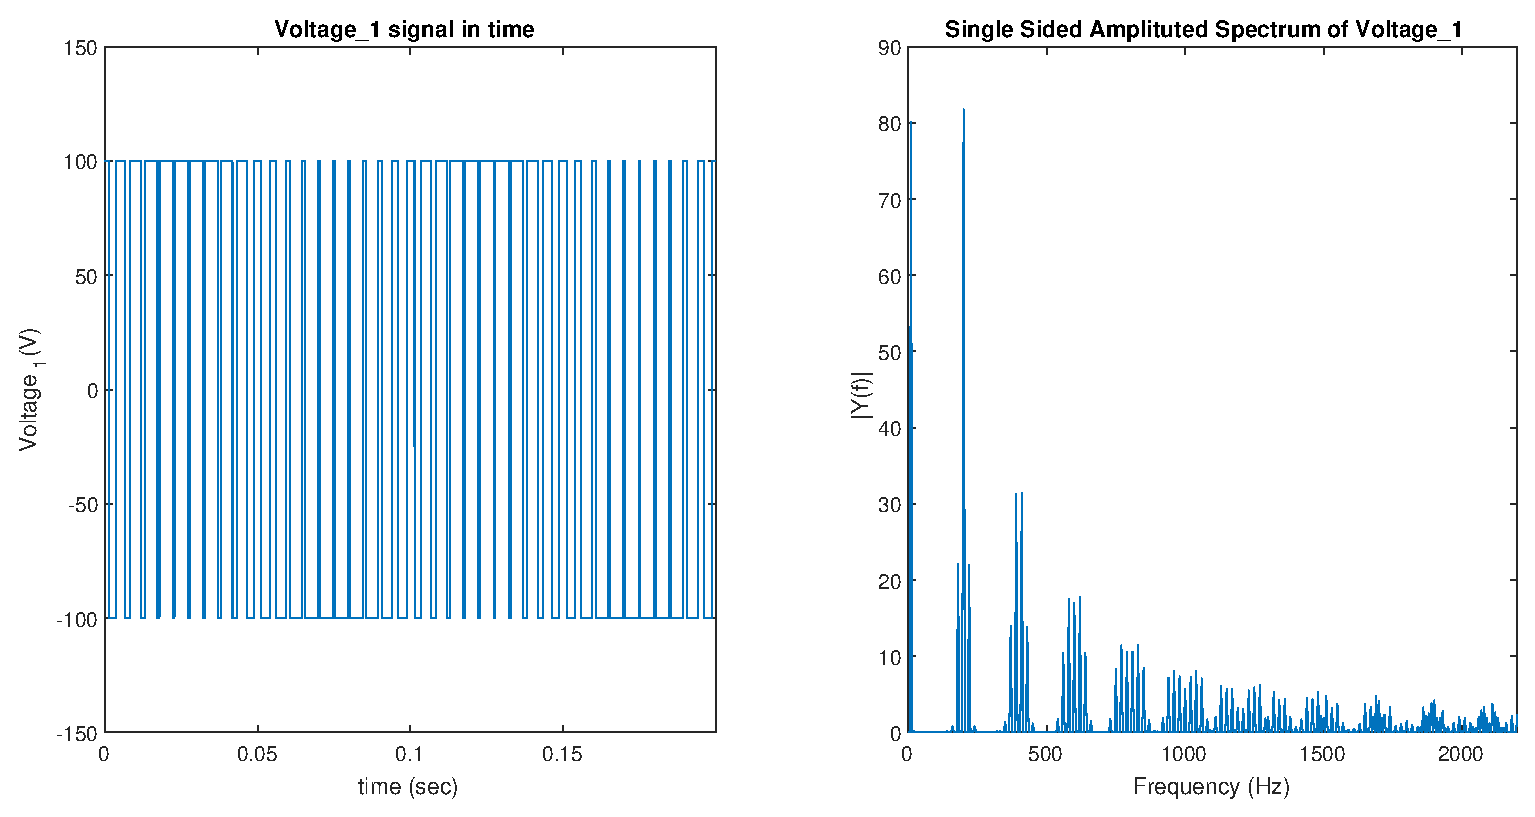
\includegraphics[width=\textwidth]{voltage1_Q3.eps} 
\end{figure} 

τι κάνεις γαμώ την παναγία σου 
	\section*{Άσκηση 3}
\label{ex3}
\addcontentsline{toc}{section}{\nameref{ex3}}

\subsection*{Ερώτημα 1}
\label{ex3q1}
\addcontentsline{toc}{subsection}{\nameref{ex3q1}}

Αναπαριστούμε τα states ως 3 αριθμοί, ο πρώτος είναι η τωρινή σελίδα και οι άλλοι 2 αριθμοί είναι οι σελίδες που είναι cached οπότε προκύπτουν 5 πιθανά states: (1,1,2) (2,1,2) (1,1,3) (3,1,3) (3,2,3) (2,2,3) και μέσω αυτών κατασκευάζεται ο πίνακας μετάβασης:


\noindent\\
Η λύση του προβλήματος προκύπτει λύνοντας τις παρακάτω σχέσεις:
\begin{align*}
    &\pi_{(3,2,3)} = \pi_{(2,2,3)}(1 - y) + \pi_{(1,1,2)}(1 - x) + \pi_{(2,1,2)}(1 - y) \\
    &\pi_{(2,2,3)} = \pi_{(3,2,3)} + \pi_{(3,1,3)} + \pi_{(1,1,3)}x \\ 
    &\pi_{(1,1,3)} = \pi_{(2,2,3)}y \\
    &\pi_{(3,1,3)} = \pi_{(1,1,3)}(1 - x)\\
    &\pi_{(2,1,2)} = \pi_{(1,1,2)}x \\
    & 1 = \pi_{(3,2,3)} + \pi_{(2,2,3)} + \pi_{(1,1,3)} + \pi_{(3,1,3)} + \pi_{(2,1,2)} + \pi_{(1,1,2)} \\
\end{align*}
 
οπότε λύνοντας τις παραπάνω σχέσει προκύπτουν οι παρακάτω τιμές:
\begin{align*}
    &\pi_{(2,1,2)} = 0 \\
    &\pi_{(1,1,2)} = 0 \\
    &\pi_{(2,2,3)} = \frac{1}{2 + y - xy}\\ 
    &\pi_{(3,1,3)} = \frac{(1-x)y}{2 + y - xy}\\
    &\pi_{(3,2,3)} = \frac{1-y}{2 + y - xy}\\
    &\pi_{(1,1,3)} = \frac{y}{2 + y - xy}\\
\end{align*}
 

\subsection*{Ερώτημα 2}
\label{ex3q2}
\addcontentsline{toc}{subsection}{\nameref{ex3q2}}


Για να βρεθεί ο αριθμός των request προς σελίδες που είναι ήδη cashed, έτσι η ζητούμενη τιμή είναι ίση με το άθροισμα όλων των request προς cashed σελίδες επί την πιθανότητα μετάβασης σε αυτή.
	\section*{Άσκηση 4}
\label{ex4}
\addcontentsline{toc}{section}{\nameref{ex4}}

\subsection*{Ερώτημα 1}
\label{ex4q1}
\addcontentsline{toc}{subsection}{\nameref{ex4q1}}

Σύμφωνα με τα δεδομένα κάθε πίνακα, είναι εμφανές πως και για το Α και για το Β η πιθανότητα να βρεθούν σε ένα οποιοδήποτε κανάλι ξεκινώντας από οποιοδήποτε κανάλι, είναι ίση $\frac{1}{3}$. Έτσι, είναι προφανές πως για να βρεθούν στο ίδιο κανάλι απαιτούνται $\frac{1}{\frac{1}{3}}$ βήματα (δηλαδή 3 βήματα) κατά μέσο όρο δηλαδή αναμένεται να υπάρχει "σύγκρουση" αν 3 βήματα κατά μέσο όρο.
\subsection*{Ερώτημα 2}
\label{ex4q2}
\addcontentsline{toc}{subsection}{\nameref{ex4q2}}
\end{document}